% =====================================================================
% Rozdział 2 – Podstawy teoretyczne i przegląd rozwiązań (~8–9 str.)
% Teoria niezależna od projektu („jak to działa w ogóle”).
% Skróty z tytułów (SoC, UDP, TCP) wyjaśnić na początku rozdziału.
% =====================================================================
\chapter{Podstawy teoretyczne i~przegląd rozwiązań}
\label{ch:teoria}

% ---------------------------------------------------------------------
\section{Mikrokontrolery i~układy SoC w~systemach wbudowanych}
\label{sec:mcu-soc}
% - Mikrokontroler, mikroprocesor i SoC (System on Chip) – różnice;
%   ESP32-S3 jako SoC.
% - Hierarchia pamięci: wewnętrzna SRAM (szybka, mała), zewnętrzna PSRAM
%   (duża, wolniejsza), flash (program, stałe, np. LUT), cache.
% - Instrukcje wektorowe (SIMD) – podstawa przyspieszenia ESP-NN.
% - DMA – przesyłanie klatek z kamery bez udziału procesora.
% - System czasu rzeczywistego (FreeRTOS): zadania, priorytety, tick.
% - Uzasadnienie: bez tych pojęć nie da się wyjaśnić wyników z
%   \ref{sec:oprogramowanie-wezla} i \ref{sec:wydajnosc}
%   (arena w PSRAM, cache 64 kB, koszt kontroli sterty).
% Stan: ✅ tekst (v2, ok. 1,5 str.); ⏳ rys. hierarchii pamięci
%       (imgs/hierarchia_pamieci.drawio.png); ⏳ sprawdzić strony w Wolfie
%       i nr podrozdz. w Hennessym; ⏳ źródło definicji PSRAM.

Węzeł kamerowy opisany w~dalszej części pracy jest systemem wbudowanym
zbudowanym na układzie SoC (ang.~\textit{System on Chip} -- system w~jednym
układzie scalonym). System wbudowany to system przetwarzania informacji
umieszczony wewnątrz większego urządzenia \cite[s.~2]{marwedel_2021}. Wykonuje
jedno, z~góry określone zadanie przy ograniczonej pamięci, mocy obliczeniowej
i~energii, często z~wymaganiami czasowymi \cite[podrozdz.~1.4]{marwedel_2021}.

\subsubsection*{Mikrokontroler i~układ SoC}

W~mikroprocesorze (ang.~\textit{microprocessor unit}, MPU) pamięć i~układy
peryferyjne są osobnymi układami scalonymi. Mikrokontroler
(ang.~\textit{microcontroller unit}, MCU) zawiera w~jednym układzie procesor,
pamięć RAM, pamięć programu oraz peryferia, takie jak liczniki, przetworniki
analogowo-cyfrowe i~interfejsy komunikacyjne \cite[podrozdz.~1.2]{wolf_2017}.
Jest przez to tani, pobiera mało energii i~reaguje na zdarzenia
w~przewidywalnym czasie. Układ SoC dokłada do tego wyspecjalizowane bloki, np.
moduł radiowy Wi-Fi, akceleratory sprzętowe lub kilka rdzeni
\cite[podrozdz.~3.3.2]{marwedel_2021}. Granica między MCU a~SoC jest umowna:
producenci opisują mikrokontrolery z~wbudowanym Wi-Fi jako SoC oparte na
mikrokontrolerze \cite{espressif_esp32s3_ds}. Do tej grupy należy ESP32-S3,
opisany w~podrozdz.~\ref{sec:wezel}.

\subsubsection*{Hierarchia pamięci}

Pamięć szybka jest droga, a~pamięć pojemna jest wolna. Dlatego organizuje się
ją w~hierarchię: im bliżej rdzenia, tym mniejsza i~szybsza
\cite[podrozdz.~2.1]{hennessy_2019}, \cite[podrozdz.~3.4.2]{marwedel_2021}.
Hierarchia działa, bo programy odwołują się najczęściej do danych używanych
przed chwilą i~do adresów sąsiednich (lokalność czasowa i~przestrzenna)
\cite[dod.~B.1]{hennessy_2019}. W~układach SoC występują zwykle cztery
poziomy pamięci (rys.~\ref{fig:hierarchia-pamieci}):
\begin{itemize}[nosep]
  \item \textbf{wewnętrzna SRAM} (ang.~\textit{static RAM}) -- setki
        kilobajtów, najszybsza; mieści stos, zmienne i~najczęściej używane
        bufory;
  \item \textbf{pamięć podręczna} (ang.~\textit{cache}) -- mała SRAM
        z~kopiami ostatnio używanych fragmentów pamięci zewnętrznych;
  \item \textbf{zewnętrzna PSRAM} (ang.~\textit{pseudo-static RAM}) --
        pamięć dynamiczna z~wbudowanym odświeżaniem, o~pojemności rzędu
        megabajtów; dołączona magistralą SPI, więc wyraźnie wolniejsza
        i~dostępna przez pamięć podręczną;
  \item \textbf{pamięć flash} -- nieulotna, mieści program i~dane stałe;
        kod wykonuje się wprost z~niej przez pamięć podręczną
        (ang.~\textit{execute in place}, XIP).
\end{itemize}
Taką organizację ma m.in. ESP32-S3 \cite[rozdz.~4]{espressif_esp32s3_trm},
\cite{espressif_idf_memtypes}.

\begin{figure}[htbp]
  \centering
  % Źródło rysunku: imgs/hierarchia_pamieci.tex (TikZ, standalone) -> PDF.
  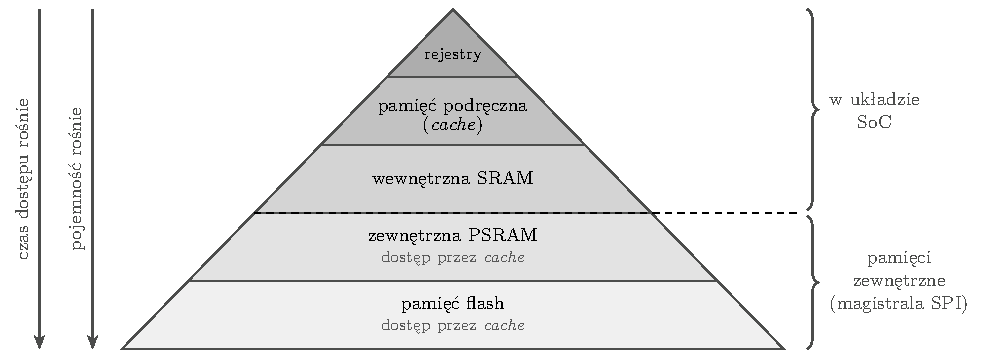
\includegraphics[width=0.85\textwidth]{imgs/hierarchia_pamieci.pdf}
  \caption{Hierarchia pamięci w~układzie SoC. Im bliżej rdzenia procesora
    (rejestry na szczycie), tym mniejsza pojemność i~krótszy czas dostępu.
    Pamięci zewnętrzne są dostępne przez pamięć podręczną (opracowanie własne
    na podstawie \cite{hennessy_2019})}
  \label{fig:hierarchia-pamieci}
\end{figure}

Gdy potrzebnych danych nie ma w~pamięci podręcznej (ang.~\textit{cache miss}),
procesor czeka, aż cała linia zostanie sprowadzona z~wolniejszej pamięci
\cite[dod.~B.1]{hennessy_2019}. Algorytmy przeglądające w~każdej klatce duże
tablice -- wagi sieci neuronowej lub tablicę przekodowań obrazu -- są więc
wrażliwe na rozmiar pamięci podręcznej i~na to, w~której pamięci leżą dane.
Widać to w~pomiarach w~podrozdz.~\ref{sec:wydajnosc}.

\subsubsection*{Instrukcje wektorowe SIMD}

Instrukcje SIMD (ang.~\textit{single instruction, multiple data}) wykonują
tę samą operację na kilku danych naraz, zapisanych w~jednym szerokim rejestrze
\cite[podrozdz.~4.3]{hennessy_2019}, \cite[podrozdz.~3.3.2]{marwedel_2021}.
Rejestr 128-bitowy mieści 16 liczb 8-bitowych, więc jedna instrukcja zastępuje
16 zwykłych. W~sieciach neuronowych podstawową operacją jest mnożenie
z~akumulacją (ang.~\textit{multiply-accumulate}, MAC): $a \leftarrow a + w
\cdot x$. SIMD przyspiesza je najbardziej, gdy dane są wąskimi liczbami
całkowitymi ułożonymi w~pamięci kolejno i~z~wyrównaniem
\cite[podrozdz.~4.3]{hennessy_2019} -- stąd znaczenie kwantyzacji do 8~bitów
(podrozdz.~\ref{sec:detekcja-mcu}).

Kod SIMD pisze się zwykle ręcznie, dlatego producenci dostarczają biblioteki
gotowych jąder obliczeniowych dla warstw sieci. Biblioteka CMSIS-NN dla
procesorów Arm Cortex-M przyspieszyła sieć splotową 4,6~razy względem
implementacji bazowej \cite[rozdz.~6]{lai_2018}. Odpowiednikiem dla układów
Espressif jest ESP-NN \cite{espressif_espnn}, która w~ESP32-S3 korzysta
z~rozszerzenia PIE (ang.~\textit{Processor Instruction Extensions})
\cite[rozdz.~1]{espressif_esp32s3_trm}.

\subsubsection*{Bezpośredni dostęp do pamięci}

Kontroler DMA (ang.~\textit{direct memory access}) przesyła dane między
peryferium a~pamięcią bez udziału procesora, który w~tym czasie może liczyć
\cite[podrozdz.~4.3]{wolf_2017}. W~systemach z~kamerą DMA przepisuje piksele
z~interfejsu kamery do bufora ramki \cite[rozdz.~3]{espressif_esp32s3_trm}.
Przy dwóch buforach kamera zapisuje nową klatkę do jednego, a~program
przetwarza klatkę z~drugiego \cite{espressif_esp32camera}. Akwizycja
i~obliczenia idą wtedy równolegle, ale przetwarzana klatka ma już swój
,,wiek'' -- od jej rejestracji minęło trochę czasu. Ten wiek wchodzi
w~opóźnienie systemu (podrozdz.~\ref{sec:wydajnosc}).

\subsubsection*{Systemy czasu rzeczywistego i~RTOS}

System czasu rzeczywistego to system, którego poprawność zależy nie tylko od
wyniku, lecz także od chwili, w~której wynik powstaje
\cite[podrozdz.~1.1]{kopetz_2011}. Według Kopetza termin
(ang.~\textit{deadline}) jest twardy, gdy jego przekroczenie może mieć poważne
skutki, oraz typu \textit{firm}, gdy spóźniony wynik jest bezużyteczny, ale
nie szkodzi \cite[podrozdz.~1.1]{kopetz_2011}. Detekcja obiektów wokół robota
należy do tej drugiej grupy: spóźniony wynik opisuje nieaktualne położenie,
więc się go odrzuca, a~po chwili przychodzi nowy. Ten argument wraca przy
wyborze protokołu w~podrozdz.~\ref{sec:protokoly}.

System operacyjny czasu rzeczywistego (ang.~\textit{real-time operating
system}, RTOS), np. FreeRTOS, dzieli program na zadania o~stałych
priorytetach. Planista uruchamia zawsze gotowe zadanie o~najwyższym
priorytecie i~wywłaszcza zadanie bieżące, gdy tylko takie się pojawi
\cite[podrozdz.~4.12.3]{barry_freertos}. Zadanie czekające na dane, np. na
element kolejki, jest zablokowane i~nie zużywa czasu procesora
\cite[podrozdz.~4.7.1, 5.2.3]{barry_freertos}. Czas w~RTOS odmierza takt
systemowy (ang.~\textit{tick}) -- okresowe przerwanie, którego częstotliwość
wyznacza rozdzielczość opóźnień \cite[podrozdz.~4.6]{barry_freertos}.
W~układach dwurdzeniowych stosuje się wariant symetryczny
(ang.~\textit{symmetric multiprocessing}, SMP), w~którym zadanie można
przypiąć do wybranego rdzenia \cite{espressif_idf_freertos}. Pozwala to
oddzielić obliczenia od obsługi sieci i~kamery
(podrozdz.~\ref{sec:oprogramowanie-wezla}).


% ---------------------------------------------------------------------
\section{Detekcja obiektów na mikrokontrolerach}
\label{sec:detekcja-mcu}
% - Detekcja obiektów (klasa + położenie) a klasyfikacja obrazu.
% - Klasyczne detektory: SSD, YOLO – prostokąty, dużo pamięci i obliczeń.
% - TinyML: ograniczenia (setki kB RAM, brak GPU, kilkaset MHz).
% - FOMO (Faster Objects, More Objects):
%   - zamiast prostokątów zwraca centroidy na siatce,
%   - wyjście: mapa komórek (96x96, redukcja 8x -> siatka 12x12),
%   - każda komórka ma prawdopodobieństwo klasy,
%   - wycięta część MobileNetV2 (bez głowy klasyfikacyjnej).
% - Zalety FOMO: wystarczy położenie (kierunek). Wady: brak rozmiaru
%   obiektu, bliskie obiekty zlewają się w jedną komórkę.
% - Porównanie z alternatywami na MCU (mniejsze YOLO, person detection
%   Espressif) – dlaczego nie one.
% - Kwantyzacja int8 (zwięźle, ok. 1 strona):
%   - float32 vs int8; kwantyzacja po treningu:
%     q = round(x/scale) + zero_point,
%   - zyski: 4x mniejszy model, arytmetyka całkowita, SIMD;
%     koszty: niewielki spadek dokładności, zbiór kalibracyjny,
%   - dlaczego na MCU int8 to praktycznie jedyny rozsądny wybór,
%   - opcjonalnie: liczba MAC (FOMO MobileNetV2 0.1, 96x96x1
%     ≈ 3,5 mln MAC – wyliczenie własne).
% - Tab.: FOMO / SSD / YOLO – wyjście, rozmiar modelu, RAM, czy mieści
%   się na MCU.
% Stan: ✅ (teoria)


% ---------------------------------------------------------------------
\section{Model kamery i~kalibracja}
\label{sec:model-kamery}
% - Model otworkowy (pinhole): rzutowanie punktu 3D na płaszczyznę obrazu.
% - Macierz parametrów wewnętrznych K: fx, fy, cx, cy.
% - Dystorsja radialna (k1, k2, k3) i styczna (p1, p2) – wzory,
%   dystorsja beczkowa/poduszkowa.
% - Parametry zewnętrzne: obrót R i przesunięcie t.
% - Kalibracja szachownicą (metoda Zhanga), minimalizacja błędu
%   reprojekcji; RMS reprojekcji jako miara jakości.
% - HFOV = 2*atan(W / (2*fx)).
% - Kierunek promienia z piksela: x_n = (u - cx)/fx -> azymut atan(x_n).
% - Rys.: model otworkowy. Rys.: przykład dystorsji beczkowej.
% Stan: ✅ (teoria)


% ---------------------------------------------------------------------
\section{Fuzja danych w~systemach wielokamerowych}
\label{sec:fuzja-teoria}
% - Po co fuzja: kilka kamer widzi ten sam obiekt w obszarach nakładania.
% - Wspólny układ odniesienia: detekcje z układu kamery -> układ robota.
% - Asocjacja danych: czy dwie detekcje to ten sam obiekt (progi kątowe,
%   odległość, czas).
% - Łączenie detekcji: średnia ważona pewnością, wybór najlepszej itp.
% - Synchronizacja czasowa: znaczniki czasu.
% - Przegląd istniejących systemów wielokamerowych (systemy dookólne
%   w samochodach, roboty mobilne) – krótko.
% Stan: ✅ (teoria)


% ---------------------------------------------------------------------
\section{Protokoły transportowe w~systemach czasu rzeczywistego}
\label{sec:protokoly}
% - Do ok. 1 strony (najłatwiejsze miejsce do skrócenia).
% - TCP: połączeniowy, potwierdzenia, retransmisje, kolejność – kosztem
%   opóźnień (head-of-line blocking).
% - UDP: datagramy bez połączenia i retransmisji, nagłówek 8 B.
% - Dlaczego UDP w czasie rzeczywistym: stary wynik detekcji jest
%   bezwartościowy – lepiej zgubić pakiet niż czekać.
% - Konsekwencje: obsługa utraty, duplikatów, kolejności po stronie
%   aplikacji (numer sekwencyjny, znacznik czasu).
% - Wi-Fi 2,4 GHz: wspólne medium, zmienne opóźnienie.
% - Tab.: TCP vs UDP.
% Stan: ✅ (teoria)